\documentclass{slides}

\usepackage{geometry}
\geometry{screen}
\usepackage{graphicx,epstopdf}

\title{How to Choose $ \delta$}
\author{(if someone hands you an $ \varepsilon$)}
\begin{document}

\maketitle

\begin{slide}
\input{slides/03epsAndNoDelta.tex}
\end{slide}

\begin{slide}

    \begin{picture} (180.000000,180.000000)(0,0)
    \put(0.0, 0.0){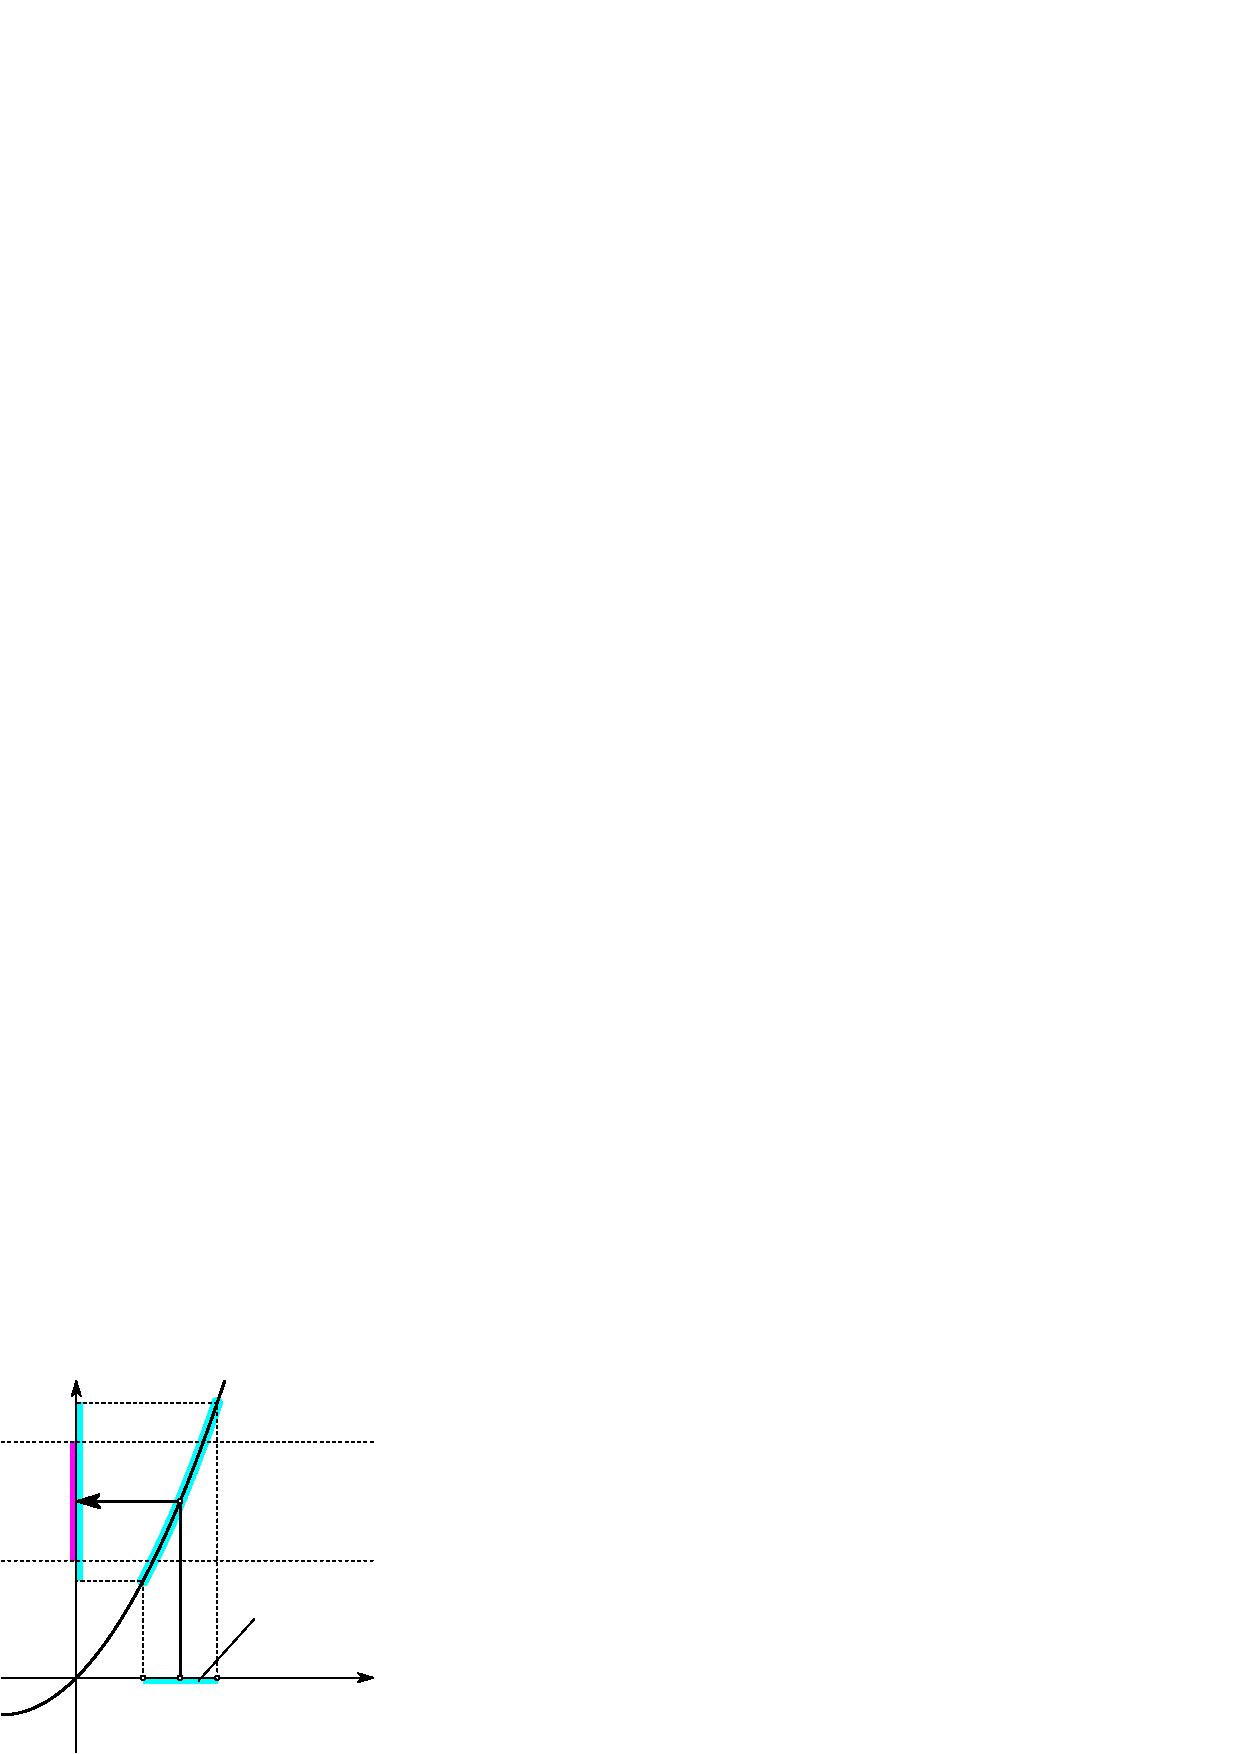
\includegraphics{03epsAndDeltaTooBig.pdf}}
        \put( -2.00,  92.85){\sffamily\itshape \makebox[0pt][r]{$L-\varepsilon$}}
    \put( -2.00, 149.81){\sffamily\itshape \makebox[0pt][r]{$L+\varepsilon$}}
    \put( 31.60, 121.33){\sffamily\itshape \makebox[0pt][r]{$L$}}
    \put(108.24, 168.50){\sffamily\itshape $y=f(x)$}
    \put(107.24,  39.60){\sffamily\itshape $a+\delta$}
    \put( 44.64,  39.60){\sffamily\itshape $a-\delta$}
    \put( 84.44,  24.60){\sffamily\itshape $a$}
    \put(125.04,  64.72){\sffamily\itshape \begin{minipage}{240pt}
        For some $x$ in this interval $f(x)$ is not between
        $L-\varepsilon$ and $L+\varepsilon$. Therefore the $\delta$ in this
        picture is too big for the given $\varepsilon$.  You need a smaller
        $\delta$.
        \end{minipage}}
\end{picture}

\end{slide}

\begin{slide}
\input{slides/03epsAndDelta.tex}
\end{slide}

\begin{slide}
How do you turn all this into equations?
\end{slide}


\end{document}
%\documentclass[12pt]{amsart}

%\usepackage{geometry}
%\geometry{screen}

%\usepackage{graphicx,epstopdf}

%
%%%% BEGIN DOCUMENT
%\begin{document}
%\null\vfill
%\begin{center}
%\textsc{\Huge How to Choose $ \delta$}\\[1in]
%(if someone hands you an $ \varepsilon$)
%\end{center}
%\vfill\newpage

%
%\input{slides/03epsAndNoDelta.tex}

%
    \begin{picture} (180.000000,180.000000)(0,0)
    \put(0.0, 0.0){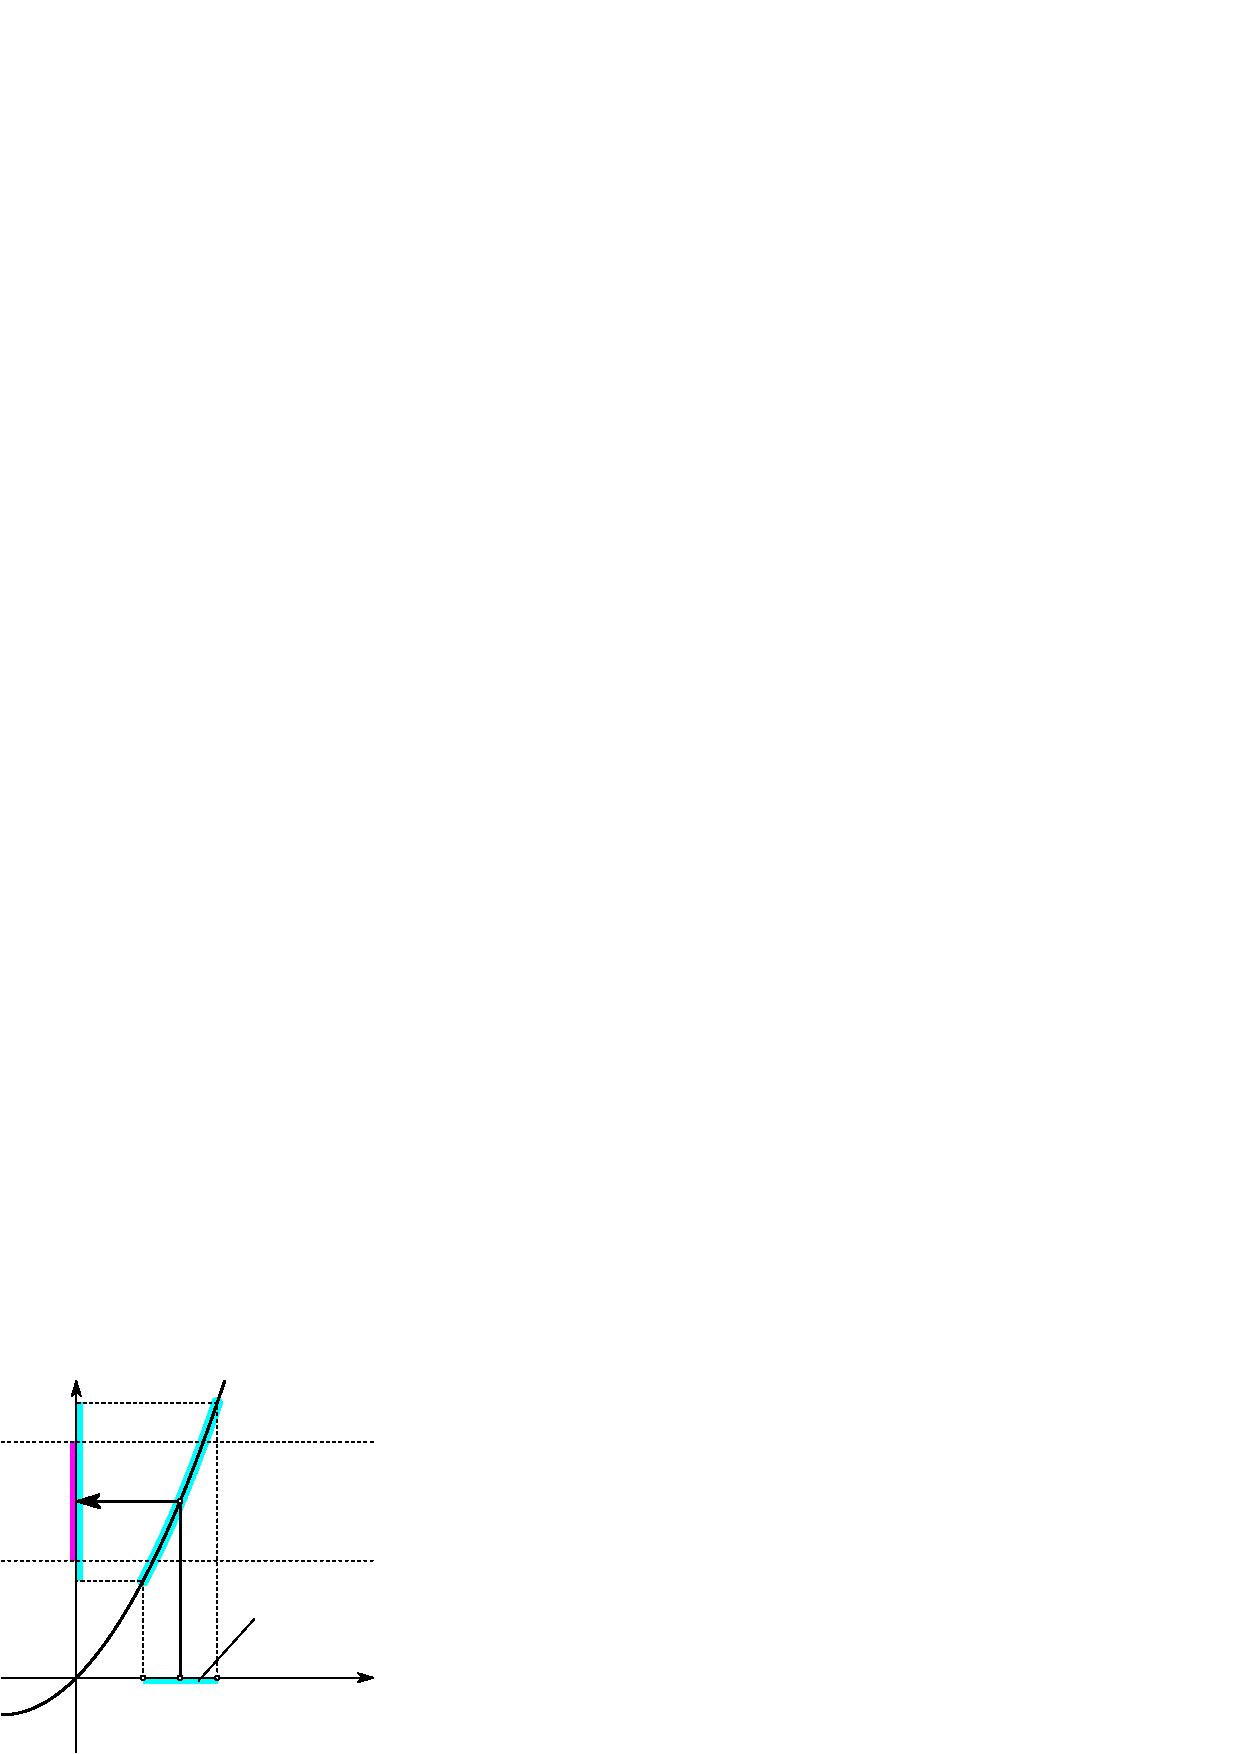
\includegraphics{03epsAndDeltaTooBig.pdf}}
        \put( -2.00,  92.85){\sffamily\itshape \makebox[0pt][r]{$L-\varepsilon$}}
    \put( -2.00, 149.81){\sffamily\itshape \makebox[0pt][r]{$L+\varepsilon$}}
    \put( 31.60, 121.33){\sffamily\itshape \makebox[0pt][r]{$L$}}
    \put(108.24, 168.50){\sffamily\itshape $y=f(x)$}
    \put(107.24,  39.60){\sffamily\itshape $a+\delta$}
    \put( 44.64,  39.60){\sffamily\itshape $a-\delta$}
    \put( 84.44,  24.60){\sffamily\itshape $a$}
    \put(125.04,  64.72){\sffamily\itshape \begin{minipage}{240pt}
        For some $x$ in this interval $f(x)$ is not between
        $L-\varepsilon$ and $L+\varepsilon$. Therefore the $\delta$ in this
        picture is too big for the given $\varepsilon$.  You need a smaller
        $\delta$.
        \end{minipage}}
\end{picture}


%\input{slides/03epsAndDelta.tex}

%

%

%

%\end{document}
